\chapter{Análisis de requisitos}

Una vez tenemos clara la descripción genérica del problema, pasemos a enfocar el problema desde un punto de vista más técnico y agrupemos los requisitos de forma previa a su desarrollo:

\section{Requisitos funcionales}

Para empezar, recopilemos las funcionalidades que deben ser implementadas en el sistema para un correcto desempeño de la aplicación previamente mencionada, dadas las características tan explícitas de ésta:

\begin{itemize}
	\item \textbf{Inicio de sesión automático:} tras cargar el sistema operativo, en lugar de mostrar una terminal o pantalla de inicio de sesión, se deberá acceder al sistema de forma automática con permisos suficientes para ejecutar y cerrar aplicaciones, montar y desmontar interfaces de disco, etc.
	\item \textbf{Ejecución de la aplicación embebida:} el sistema ha de tener el ejecutable del programa instalado en un directorio accesible, con permisos de ejecución para el usuario por omisión.
	\item \textbf{Soporte para conectividad:} la infraestructura a desarrollar debe tener instaladas las dependencias necesarias para proveer al código de la aplicación de binarios útiles para administrar las interfaces de red y sus estados, además de listar las redes disponibles y poder establecer una conexión con éstas.
	\item \textbf{Soporte de almacenamiento externo:} el sistema debe detectar en todo momento que se ha insertado un dispositivo externo, haciendo lo necesario para su montaje y su puesta a punto para el uso de la aplicación. Para esto, será imprescindible que acepte la mayoría de los formatos convencionales actualmente (\textit{NTFS, FAT, exFAT} y \textit{EXTx} entre otros).
\end{itemize}

Vistos dichos requisitos, examinemos los requerimientos de la infraestructura externos a la aplicación, como lo es el \textbf{servicio de actualizaciones}:

\begin{itemize}
	\item El paradigma de despliegue de versiones debe ser fácil de acoplar al sistema y transparente con la aplicación, de forma que ésta sea consciente de la existencia de nuevas versiones y pueda pedir confirmación al usuario. Además, deberán estar centralizadas en un servidor (ya sea local a la empresa o contratado de forma externa); de forma que en lugar de enviarse la actualización individualmente a cada máquina, sean las propias máquinas las que mediante la comunicación con el servidor detecten las potencialmente nuevas versiones.
	\item Para poder realizar actualizaciones atómicas de todo el sistema, será necesario un particionado múltiple. Es decir, el mismo sistema operativo deberá tener dos particiones con sistema de ficheros. Así, mientras una está en ejecución la nueva versión podrá ser instalada en la otra.
	\item Este intercambio de información podrá producirse mediante red cableada o inalámbrica, sin que ello importe al resultado de la operación o dificulte este proceso.
	\item En cada nueva versión del sistema operativo, deberán incluirse las nuevas versiones tanto de la aplicación como del software de la \textbf{electrónica interna} (que se manejaría íntegramente por la aplicación embebida y no ya por la distro en cuestión).
\end{itemize}

Vistas las necesidades del sistema de actualización, veamos ahora un diagrama de estados con el proceso:

\begin{figure}[H]
	\centering
	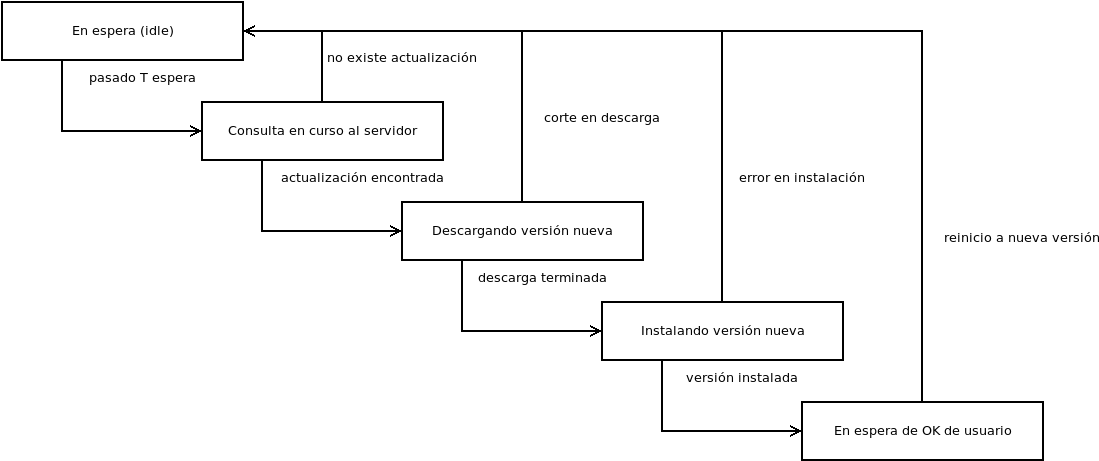
\includegraphics[width=\linewidth]{imagenes/statechart-actualizacion.png}
	\caption{Diagrama de estados del proceso de actualización}
	\label{statechart-actualizacion}
\end{figure}

Una vez definido a petición un período de comprobación de versiones, el cliente se mantendrá a la espera hasta que dicho período se dispare; entonces realizará mediante HTTPS una consulta al servidor, quien le responderá si existe una versión nueva o no.\\

Si no la hay, el cliente vuelve a \textit{``dormirse''}. De lo contrario, comienza la descarga en segundo plano del nuevo software; el cual es instalado en la partición inactiva.\\

Una vez que el usuario da su aprobación mediante la interfaz de la aplicación, o bien cuando decide reiniciar/apagar voluntariamente; la partición marcada como ``activa'' deja de ser la primera. Esto ocasiona que el próximo arranque de la máquina se realice cargando el software más nuevo.\\

Si se produce algún error que impide lanzar la \textit{nueva distro}, o por cualquier motivo no se consigue conectar con el servidor para notificar la actualización realizada, se considera errónea o fallida, volviendo a marcarse la partición antigua como activa y reiniciando al sistema de ficheros antiguo.

\section{Requisitos no funcionales}

Ahora bien, pasemos a ver por otro lado los requerimientos relacionados con las especificaciones de rendimiento, estabilidad, disponibilidad y aspectos estéticos.

\begin{itemize}
	\item En cuanto al \textbf{rendimiento} del sistema, todas las prestaciones de la infraestructura deben centrarse en las acciones del usuario, respondiendo rápido a la interacción táctil, procesando los cálculos internos (de medidas, actualización de gráficas) de manera fluida y eficiente, con los requerimientos de procesamiento gráfico que ello conlleve.
	\item Además, otra parte del rendimiento será el \textit{tiempo de encendido}. Cuanto más ligero sea el sistema operativo y menos (idealmente cero) procesos innecesarios contenga, menor será dicha magnitud. Adicionalmente, la aplicación deberá ser de los primeros servicios en lanzarse, de forma previa al resto de procesos, que lo harán en segundo plano.
	\item Desde el punto de vista de \textbf{la seguridad}, es necesario blindar al sistema intrínseco de cualquier manipulación externa, por lo que el sistema operativo debe ser consciente de si se está ejecutando o no la aplicación en un servicio dedicado, tomando medidas de recuperación cuando no esté haciéndolo (como la re-ejecución del proceso o el reinicio de la máquina). Además, deberá establecerse un proceso que detecte en segundo plano si se ha detectado un teclado, ya que no es de utilidad para la aplicación y cualquier manipulación puede poner en peligro la estabilidad del sistema.
	\item Otro aspecto de la seguridad tiene que ver con las actualizaciones. El motor que las aplique debe controlar de forma exhaustiva cuándo son aplicados correctamente los despliegues, retornando a la versión anterior si no fuese capaz de informar al servidor del éxito en la operación.
	\item Para terminar con los aspectos de protección y recuperación, deberá incluirse en el dispositivo un servidor de administración (del tipo \textit{Secure SHell}) que permita al equipo de desarrollo depurar los posibles errores, así como hacer evaluaciones de rendimiento externas.
	\item Por otro lado, en el apartado \textbf{estético} y pensando en la \textit{computación ubica moderna}, es de imperativa necesidad que el sistema no muestre al usuario los mensajes de la carga que se esté produciendo, ni un modo \textit{línea de comandos} de ningún tipo, de forma que la interfaz sea \textbf{lo más natural posible}. Para ello, deberá modificarse el \textit{bootloader} del computador elegido para que silencie estos mensajes de la salida estándar; además de incluir por otro lado el sistema un servicio que imprima una imagen a pantalla completa, que será reemplazada por la aplicación.
\end{itemize}

Una vez vistos los requerimientos y funcionalidades necesarias del proyecto, pasemos ahora a enumerar y describir los actores involucrados en la vida de dicho producto.

\section{Actores}

Según \textit{Bruce Powel Douglass}, un actor no es más que un objeto (no ya siempre usuarios humanos) fuera del ámbito del sistema bajo estudio, pero que tiene una interacción directa con él \cite{real-time-uml-use-cases}. Por tanto, deberemos ser conscientes de todos los elementos involucrados en el desempeño del proyecto:

\subsubsection{Usuario normal (cliente)}

Es aquel que adquiere la máquina DYNAsystem (o la utiliza en algún gimnasio o centro). Su actuación con respecto a la máquina desde el punto de vista del sistema operativo será sencilla, ya que él simplemente llegará al dispositivo, lo encenderá y visualizará una imagen de carga hasta que aparezca la aplicación embebida, con la que podrá trabajar. Sin embargo, a lo largo de este uso utilizará indirectamente funcionalidades provistas por el sistema operativo, como la reproducción de sonidos indicativos, el guardado de datos a través de USB o la conexión WiFi. Todos estos servicios deberán ser satisfechos por el sistema.

\subsubsection{Programador(es) de la aplicación embebida}

Aunque no participan directamente en esta parte del proyecto (\textit{Meta-DYNAsystem}), para modularizar tareas y que la distribución GNU/Linux siga un desarrollo independiente será necesario el proceso de creación de la aplicación embebida por otro lado, llevado a cabo por el número de personas que la compañía estime necesarias.\\

Estos serán los encargados de abstraerse del sistema Linux y utilizar los módulos provistos por este (de gestión de interfaces de red y de discos, principalmente).

\subsubsection{Administrador(es) del sistema operativo}

Será aquel encargado de analizar, programar y compilar las nuevas versiones del sistema operativo, empaquetando las versiones de la aplicación embebida y el resto del software que se necesite incluir. Para el caso que nos ocupa, dicho puesto lo conformo yo.

\subsubsection{Servidor de actualizaciones}
	
Será el ordenador donde se centralizará todo el servicio de actualizaciones. En este deberán alojarse las imágenes compiladas y será con el que se comuniquen las máquinas (a modo de cliente) para consultar la existencia de nuevas versiones de software.\\

Dependiendo de la implementación del sistema, podrá estar situado en la oficina de la empresa o subcontratado a alguna otra compañía dedicada a la oferta de este tipo de servicios.
	
\newpage
